% This file was created by matlab2tikz.
%
%The latest updates can be retrieved from
%  http://www.mathworks.com/matlabcentral/fileexchange/22022-matlab2tikz-matlab2tikz
%where you can also make suggestions and rate matlab2tikz.
%
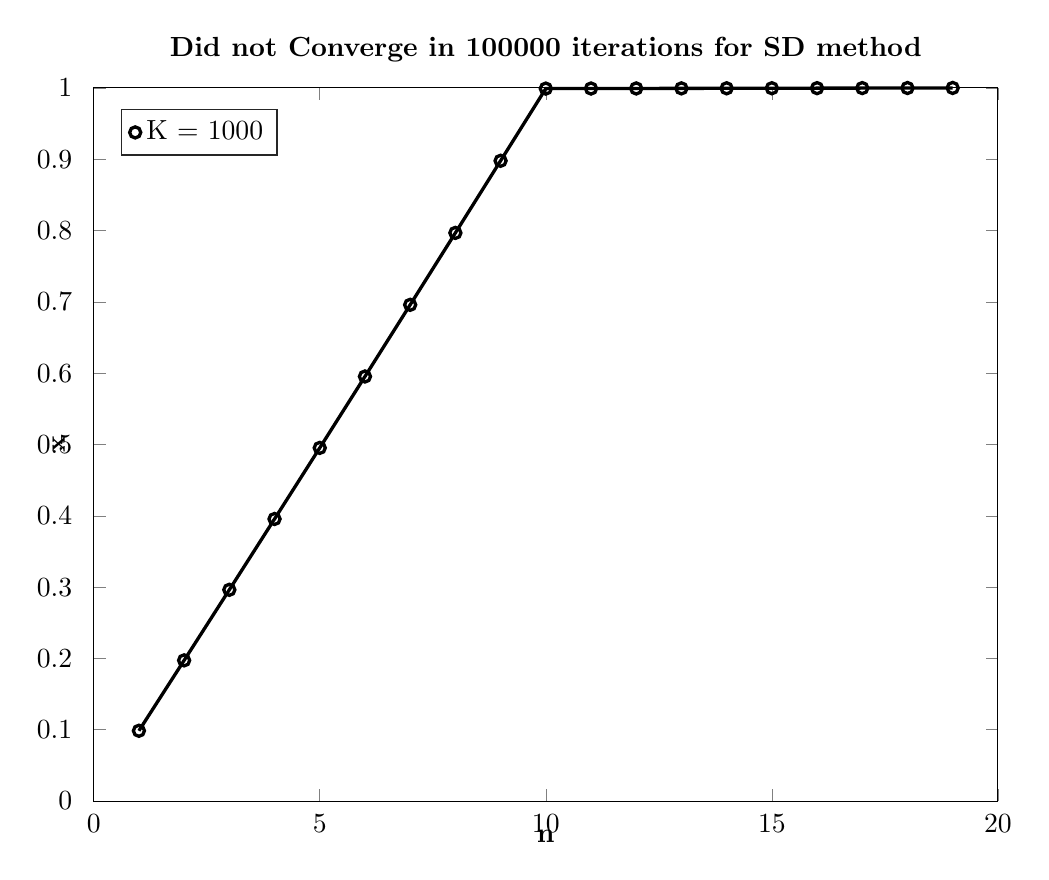
\begin{tikzpicture}

\begin{axis}[%
width=4.521in,
height=3.566in,
at={(0.758in,0.481in)},
scale only axis,
clip=false,
xmin=0,
xmax=20,
xtick={0,5,10,15,20},
xticklabels={\empty},
xlabel style={font=\bfseries},
xlabel={n},
ymin=0,
ymax=1,
ytick={0,0.1,0.2,0.3,0.4,0.5,0.6,0.7,0.8,0.9,1},
yticklabels={\empty},
ylabel style={font=\bfseries},
ylabel={x},
axis background/.style={fill=white},
title style={font=\bfseries},
title={Did not Converge in 100000 iterations for SD method},
legend style={at={(0.03,0.97)},anchor=north west,legend cell align=left,align=left,draw=white!15!black}
]
\addplot [color=black,line width=1.2pt,only marks,mark=o,mark options={solid}]
  table[row sep=crcr]{%
1	0.098574404248251\\
2	0.197278322992191\\
3	0.296228617794975\\
4	0.395518080465033\\
5	0.495206367701862\\
6	0.595314172855258\\
7	0.695821204207613\\
8	0.796668167318109\\
9	0.897762557784376\\
10	0.998987714153875\\
11	0.999088879532683\\
12	0.999190223824404\\
13	0.999291290539532\\
14	0.999392712900209\\
15	0.999493736705911\\
16	0.999595169616733\\
17	0.999696221765458\\
18	0.999797594538077\\
19	0.999898736839354\\
};
\addlegendentry{K = 1000};

\addplot [color=black,solid,line width=1.2pt,forget plot]
  table[row sep=crcr]{%
1	0.098574404248251\\
2	0.197278322992191\\
3	0.296228617794975\\
4	0.395518080465033\\
5	0.495206367701862\\
6	0.595314172855258\\
7	0.695821204207613\\
8	0.796668167318109\\
9	0.897762557784376\\
10	0.998987714153875\\
11	0.999088879532683\\
12	0.999190223824404\\
13	0.999291290539532\\
14	0.999392712900209\\
15	0.999493736705911\\
16	0.999595169616733\\
17	0.999696221765458\\
18	0.999797594538077\\
19	0.999898736839354\\
};
\node[align=center, text=black]
at (axis cs:0,-0.031) {$0$};
\node[align=center, text=black]
at (axis cs:5,-0.031) {$5$};
\node[align=center, text=black]
at (axis cs:10,-0.031) {$10$};
\node[align=center, text=black]
at (axis cs:15,-0.031) {$15$};
\node[align=center, text=black]
at (axis cs:20,-0.031) {$20$};
\node[left, align=right, text=black]
at (axis cs:-0.258,0) {$0$};
\node[left, align=right, text=black]
at (axis cs:-0.258,0.1) {$0.1$};
\node[left, align=right, text=black]
at (axis cs:-0.258,0.2) {$0.2$};
\node[left, align=right, text=black]
at (axis cs:-0.258,0.3) {$0.3$};
\node[left, align=right, text=black]
at (axis cs:-0.258,0.4) {$0.4$};
\node[left, align=right, text=black]
at (axis cs:-0.258,0.5) {$0.5$};
\node[left, align=right, text=black]
at (axis cs:-0.258,0.6) {$0.6$};
\node[left, align=right, text=black]
at (axis cs:-0.258,0.7) {$0.7$};
\node[left, align=right, text=black]
at (axis cs:-0.258,0.8) {$0.8$};
\node[left, align=right, text=black]
at (axis cs:-0.258,0.9) {$0.9$};
\node[left, align=right, text=black]
at (axis cs:-0.258,1) {$1$};
\end{axis}
\end{tikzpicture}%